\section{Tervezési minták}

\subsection{Iterátorok}

\begin{frame}
    \begin{description}[m]
        \item[Tervezési minta (design pattern)] \hfill \\ ,,Az informatikában programtervezési mintának (angolul Software Design Patterns) nevezik a gyakran előforduló programozási feladatokra adható általános, újrafelhasználható megoldásokat. Egy programtervezési minta rendszerint egymással együttműködő objektumok és osztályok leírása.''\hiv{\href{https://hu.wikipedia.org/wiki/Programtervez\%C3\%A9si_minta}{*}}
        \item[Első jelentős irodalom] \hfill \\ Erich Gamma, Richard Helm, Ralph Johnson, John Vlissides: Design Patterns (\emph{Elements of Reusable Object-Oriented Software}), Addison-Wesley, 1994
    \end{description}
\end{frame}

\begin{frame}
    \begin{description}[m]
        \item[A szerzők által meghatározott kategóriák] \hfill \\ 
            \begin{itemize}
                \item Létrehozási minták
                \item Szerkezeti minták
                \item Viselkedési minták
                    \begin{description}[m]
                        \item[Iterátor] \hfill \\ ,,Az Iterátor (\dots) minta lényege, hogy segítségével szekvenciálisan érhetjük el egy aggregált objektum elemeit, a mögöttes megvalósítás megismerése nélkül.''\hiv{\href{https://hu.wikipedia.org/wiki/Iterator_programtervez\%C3\%A9si_minta}{*}}
                    \end{description}
            \end{itemize}
    \end{description}
\end{frame}

\begin{frame}
    \begin{center}
        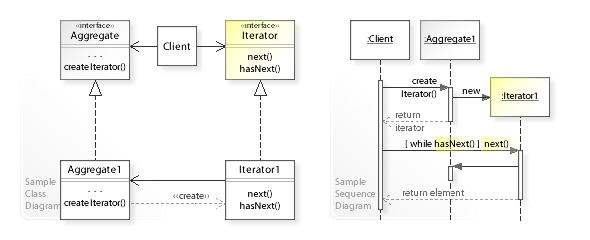
\includegraphics[width=\textwidth]{iterator.jpeg} \\
        \tiny \hiv{\href{https://upload.wikimedia.org/wikipedia/commons/c/c5/W3sDesign_Iterator_Design_Pattern_UML.jpg}{Forrás}}
    \end{center}
\end{frame}

\subsection{Iterátor példa}

\begin{frame}
    Feladat:
    \begin{itemize}
        \item Készítsünk saját iterátor interfészt, és azt megvalósító tényleges iterátorokat, melyekkel bejárható egy karakterlánc összes betűje, vagy egy láncolt lista elemei!
        \item A megvalósítás során törekedjünk a C/C++ programozók által jól ismert, mutatókhoz kapcsolódó operátorok alkalmazására!
        \begin{description}[m]
            \item[\texttt{hasNext()}] \hfill \\ \texttt{operator!=} $\to$ két iterátor ugyanazt az elemet teszi-e elérhetővé?
            \item[\texttt{next()}] \hfill \\ \texttt{operator++} $\to$ iterátor léptetése a következő elemre
                                          \\ \texttt{operator*} $\to$ az iterátor által kijelölt elem lekérése
        \end{description}
    \end{itemize}
\end{frame}

\begin{frame}
    \begin{exampleblock}{\textattachfile{Iterator.h}{Iterator.h}}
        \lstinputlisting[language=C++,linerange={4-10},numbers=left,firstnumber=4]{Iterator.h}
    \end{exampleblock}
\end{frame}

\begin{frame}
    \begin{description}[m]
        \item[\texttt{operator++}] \hfill \\ A postfix alak operátorának felültöltése:\\ \texttt{virtual Iterator operator++(\kiemel{int}) = 0;} \\
            Probléma: absztrakt osztály nem példányosítható $\to$ a visszatérési érték típusa nem lehet \texttt{Iterator}! 
    \end{description}
\end{frame}

\begin{frame}
    \begin{exampleblock}{\textattachfile{Message5.h}{Message5.h}}
        \lstinputlisting[language=C++,linerange={3-12},numbers=left,firstnumber=3]{Message5.h}
    \end{exampleblock}
\end{frame}

\begin{frame}
    \begin{exampleblock}{\textattachfile{Message5.h}{Message5.h}}
        \small
        \lstinputlisting[language=C++,style=C++,linerange={13-25},numbers=left,firstnumber=13]{Message5.h}
    \end{exampleblock}
\end{frame}

\begin{frame}
    \begin{description}[m]
        \item[\hiv{\href{https://en.cppreference.com/w/cpp/language/override}{\texttt{override}}}] \hfill \\ Azt állítjuk, hogy a tagfüggvény (felül)definiálja az öröklött függvényt $\to$ ha nem így van (pl. elgépelés), akkor hibaüzenettel leáll a fordítás.
        \item[\hiv{\href{https://en.cppreference.com/w/cpp/language/static_cast}{\texttt{static\_cast}}}] \hfill \\ Az implicit és a felhasználó által definiált típuskonverzió kombinációja, szükség esetén hívja a konverziós konstruktort. \emph{Fordítási időben} ellenőrzi a típusokat és eldönti, hogy az átalakítás végrehajtható-e. Használható primitív típusok közötti átalakításhoz, a származtatási hierarchiában történő fel- és lefelé lépéshez, vagy \texttt{void} mutatóról/ra történő konverzióhoz is.
    \end{description}
\end{frame}

\begin{frame}
    \begin{exampleblock}{\textattachfile{Message5.h}{Message5.h}}
        \scriptsize
        \lstinputlisting[language=C++,style=C++,linerange={28-42},numbers=left,firstnumber=28]{Message5.h}
    \end{exampleblock}
\end{frame}

\begin{frame}
    \begin{exampleblock}{\textattachfile{Message5.h}{Message5.h}}
        \scriptsize
        \lstinputlisting[language=C++,style=C++,linerange={44-59},numbers=left,firstnumber=44]{Message5.h}
    \end{exampleblock}
\end{frame}

\begin{frame}
    \hiv{\href{https://en.cppreference.com/w/cpp/error/out_of_range}{\texttt{std::out\_of\_range}}}
    \begin{center}
        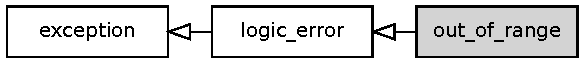
\includegraphics[scale=.6]{outofrange.pdf}
    \end{center}
    \begin{exampleblock}{\textattachfile{Message5.h}{Message5.h}}
        \scriptsize
        \vspace{-.2cm}
        \lstinputlisting[language=C++,style=C++,linerange={61-72},numbers=left,firstnumber=61]{Message5.h}
        \vspace{-.2cm}
    \end{exampleblock}
\end{frame}

\begin{frame}
    \begin{exampleblock}{\textattachfile{Message5.cpp}{Message5.cpp}}
        \small
        \vspace{-.2cm}
        \lstinputlisting[language=C++,style=C++,linerange={3-15},numbers=left,firstnumber=3]{Message5.cpp}
        \vspace{-.2cm}
    \end{exampleblock}
\end{frame}

\begin{frame}
    \begin{exampleblock}{\textattachfile{LinkedList.h}{LinkedList.h}}
        \footnotesize
        \lstinputlisting[language=C++,style=C++,linerange={3-16},numbers=left,firstnumber=3]{LinkedList.h}
    \end{exampleblock}
\end{frame}

\begin{frame}
    \begin{exampleblock}{\textattachfile{LinkedList.h}{LinkedList.h}}
        \footnotesize
        \lstinputlisting[language=C++,style=C++,linerange={18-30},numbers=left,firstnumber=18]{LinkedList.h}
    \end{exampleblock}
\end{frame}

\begin{frame}
    \begin{exampleblock}{\textattachfile{LinkedList.h}{LinkedList.h}}
        \lstinputlisting[language=C++,style=C++,linerange={32-40},numbers=left,firstnumber=32]{LinkedList.h}
    \end{exampleblock}
\end{frame}

\begin{frame}
    \begin{exampleblock}{\textattachfile{LinkedList.h}{LinkedList.h}}
        \small
        \lstinputlisting[language=C++,style=C++,linerange={42-48},numbers=left,firstnumber=42]{LinkedList.h}
    \end{exampleblock}
\end{frame}

\begin{frame}
    \begin{exampleblock}{\textattachfile{LinkedList.h}{LinkedList.h}}
        \small
        \lstinputlisting[language=C++,style=C++,linerange={50-59},numbers=left,firstnumber=50]{LinkedList.h}
    \end{exampleblock}
\end{frame}

\begin{frame}
    \begin{exampleblock}{\textattachfile{LinkedList.h}{LinkedList.h}}
        \lstinputlisting[language=C++,style=C++,linerange={61-68},numbers=left,firstnumber=61]{LinkedList.h}
    \end{exampleblock}
\end{frame}

\begin{frame}
    \begin{exampleblock}{\textattachfile{iteratorMain.cpp}{iteratorMain.cpp}}
        \small
        \lstinputlisting[language=C++,style=C++,linerange={1-12},numbers=left,firstnumber=1]{iteratorMain.cpp}
    \end{exampleblock}
\end{frame}

\begin{frame}
    \begin{exampleblock}{\textattachfile{iteratorMain.cpp}{iteratorMain.cpp}}
        \footnotesize
        \lstinputlisting[language=C++,style=C++,linerange={14-27},numbers=left,firstnumber=14]{iteratorMain.cpp}
    \end{exampleblock}
\end{frame}

\begin{frame}[fragile]
    \begin{exampleblock}{\textattachfile{iteratorMain.cpp}{iteratorMain.cpp}}
        \scriptsize
        \lstinputlisting[language=C++,style=C++,linerange={29-35},numbers=left,firstnumber=29]{iteratorMain.cpp}
    \end{exampleblock}
    \begin{block}{Kimenet}
        \vspace{-.3cm}
        \scriptsize
        \begin{verbatim}
Hello C++ world!
Hello C++ world!
Hello C++ world!
Exception caught: Message::operator[]
1	2	3          
\end{verbatim}
    \vspace{-.3cm}
    \end{block}
\end{frame}

\subsection{Iterálás tartományokon}

\begin{frame}
    \hiv{\href{https://en.cppreference.com/w/cpp/language/range-for}{Range-based for loop}} (C++11)
    \begin{itemize}
        \item Bejárhatók vele tömbök,
        \item iterátort (\texttt{begin()}, \texttt{end()}) biztosító \emph{gyűjtemények} (ld. később),
        \item és kapcsos zárójelek között felsorolt értékek.
        \item A soron következő elem elérhető érték szerint és referenciával is.
    \end{itemize}
\end{frame}

\begin{frame}
    \begin{exampleblock}{\textattachfile{range.cpp}{range.cpp}}
        \scriptsize
        \lstinputlisting[language=C++,style=C++,linerange={3-18},numbers=left,firstnumber=3]{range.cpp}
    \end{exampleblock}
\end{frame}

\begin{frame}
    \begin{exampleblock}{\textattachfile{range.cpp}{range.cpp}}
        \scriptsize
        \lstinputlisting[language=C++,style=C++,linerange={20-34},numbers=left,firstnumber=20]{range.cpp}
    \end{exampleblock}
\end{frame}

\begin{frame}
    Az \hiv{\href{https://en.cppreference.com/w/cpp/types/size_t}{\texttt{std::size\_t}}} típus
    \begin{itemize}
        \item Előjel nélküli egész típus, ami tetszőlegesen nagy objektum méretét ($\to$ \texttt{sizeof}) képes megadni bájtokban mérve.
        \item Általában indexelésre és ciklusszámlálóként használják az ilyen típusú változókat. 
    \end{itemize}
\end{frame}

\subsection{C++ iterátorok}

\begin{frame}
    \begin{description}[m]
        \item[C++ iterátorok] \hfill \\ ,,Iterátor bármely olyan objektum, amely adatok (például egy tömb vagy egy gyűjtemény) valamely elemére mutatva operátorok egy halmazának (ami legalább a növelő (\texttt{++}) és indirekció \texttt{*} műveleteket tartalmazza) segítségével képes az adatok között iterálni.''\hiv{\href{https://cplusplus.com/reference/iterator/}{*}} \\
        A legkézenfekvőbb iterátor típus a \emph{mutató}, de az összetett adatszerkezetek általában bonyolultabb megoldásokat igényelnek.
    \end{description}
\end{frame}

\begin{frame}
    Minden iterátor közös jellemzői:
    \begin{itemize}
        \item Azonos típusú értékből vagy referenciából másolással létrehozható (copy constructible).
        \item Azonos típusú érték vagy referencia hozzárendelhető (copy assignable).
        \item Megsemmisíthatő (destructible), azaz skalár típus (felültöltés nélkül is értelmezhető rajta az összeadás művelet) vagy elérhető destruktorral rendelkező osztály, melynek minden nem statikus tagja is megsemmisíthető.
        \item Értelmezett rajta a növelés (\texttt{++}) operátor (prefix és suffix alakban is).
    \end{itemize}
\end{frame}

\begin{frame}
    Kategóriák:
    \begin{description}[m]
        \item[Input] \hfill \\ Csak olvasási célra, azaz \emph{jobbértékként} indirekcióval (\texttt{*}, \texttt{->}) elérhető a mutatott adat, támogatja az egyenlőségi (\texttt{==}, \texttt{!=}) operátorokat.
        \item[Output] \hfill \\ Csak írási célra, azaz \emph{balértékként} elvégezhető rajta az indirekció, majd a hozzárendelés.
        \item[Forward] \hfill \\ Rendelkezik az input iterátorok képességeivel, és ha módosítható, akkor az output iterátorokéval is. Paraméterek vagy inicializáló értékek nélkül is létrehozható (default constructible). A szabványos gyűjtemények legalább ezt a típust megvalósítják.
    \end{description}
\end{frame}

\begin{frame}
    \begin{description}[m]
        \small
        \item[Bidirectional] \hfill \\ A Forward iterátorok képességein túl a csökkentés (\texttt{-{-}}) operátort is támogatja, bejárás hátrafelé.
        \item[Random access] \hfill \\ Mint Bidirection, de támogatja még az összeadást (\texttt{+}, \texttt{+=}), kivonást (\texttt{-}, \texttt{-=}), az egyenlőtlenségi relációkat (\texttt{<}, \texttt{<=}, \texttt{>}, \texttt{>=}) és az indexelést (\texttt{[]}) is. 
    \end{description}
    \begin{exampleblock}{\textattachfile{range.cpp}{range.cpp}}
        \scriptsize
        \lstinputlisting[language=C++,style=C++,linerange={36-41},numbers=left,firstnumber=36]{range.cpp}
    \end{exampleblock}
\end{frame}
